\pagestyle{ima}
\label{ima}

\begin{textblock*}{5.625in}(0pt,0pt)%
\vspace*{-1.45cm}
\hspace*{-1.2cm}\includegraphics*[width=112mm]{./imgs/IMA.png}
\end{textblock*}

\pagebreak

\hspace{.5cm}

\begin{center}
\hspace*{-.5cm}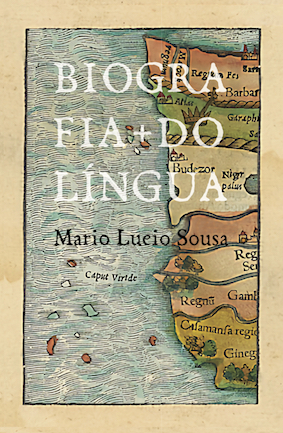
\includegraphics[width=44mm]{./imgs/lingua.jpg}
\end{center}

\hspace*{-7cm}\hrulefill\hspace*{-7cm}

\medskip

\noindent{}O último desejo de um condenado à morte é contar a vida do Língua, escravo prodigioso obrigado às mais degradantes atividades que poderia exercer: traduzir falas dos brancos nos navios negreiros para povos da África. Enquanto se desfia a biografia, pessoas se aproximam para ouvir e acabam por escrever juntas a história de um lugar, atravessando colônia, de independência e revolução. A ficção foi inspirada, segundo o autor cabo-verdiano Mário Lucio Sousa, em um homem real, entrevistado pelo etnólogo Miguel Barnet em 1963.

%\hspace{.5cm}
\vfill

\hspace*{-.4cm}\begin{minipage}[c]{1\linewidth}
\small{
{\Formular{\textbf{
\hspace*{-.1cm}Título: Biografia do Língua\\
Autor: Mario Lucio Sousa\\ 
Páginas: 302\\
Formato: 14x21cm\\
Preço: R\$ 54,00\\
ISBN: 978-85-5494-612-8\\
Disponibilidade: Em breve
}}}}
\end{minipage}

\pagebreak

\hspace{.5cm}

\begin{center}
\hspace*{-2.5cm}\raisebox{5.5cm}{\rotatebox[origin=t]{90}{\Formular{\textbf{Lançamento}}}}
\hspace*{2cm}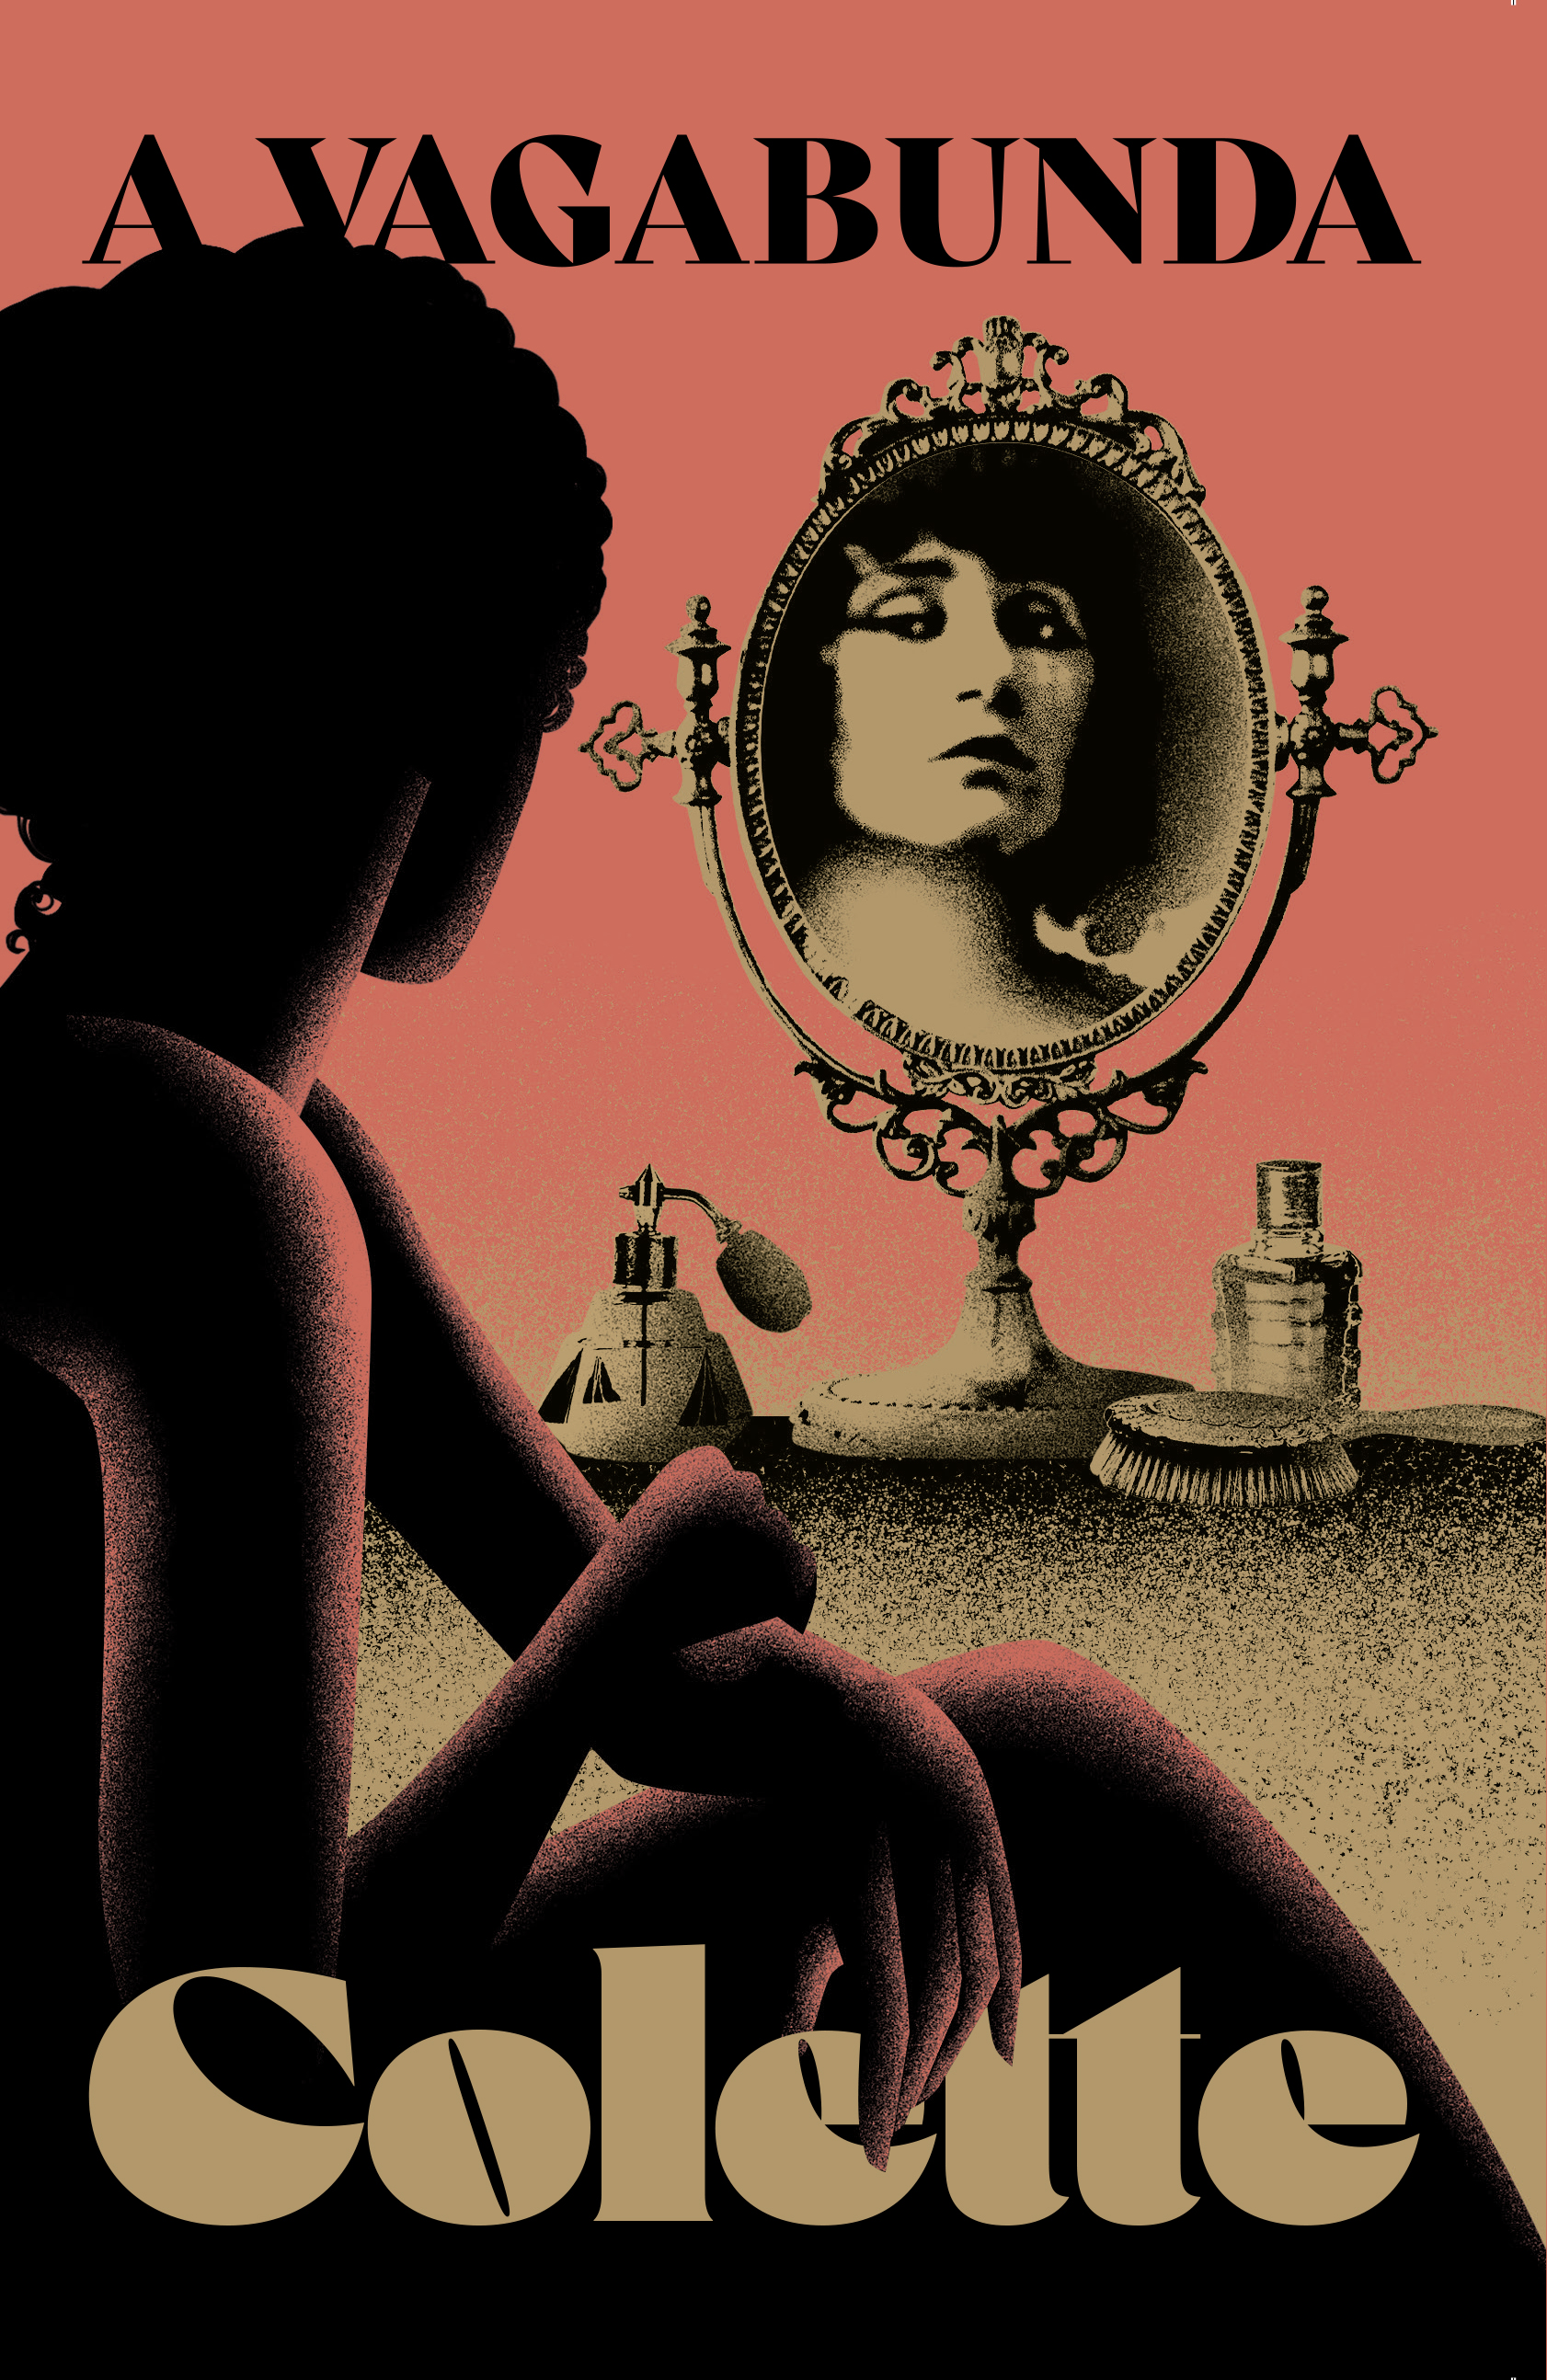
\includegraphics[width=45.8mm]{./imgs/vagabond.jpg}
\end{center}

\hspace*{-7cm}\hrulefill\hspace*{-7cm}

\medskip

\noindent{}Em {\slsc{A vagabunda}}, a indicada ao Nobel Gabrielle Sidonie Colette mistura sua vida pessoal à da protagonista, uma mulher recém"-divorciada de um homem que a traía e roubava a autoria de seus livros. A busca pela independência de Renée, trabalhando nos palcos do {\slsc{bas fond}} parisiense, configuram o enredo da obra, “um dos mais verdadeiros retratos dos dilemas de uma mulher livre em uma sociedade dominada pelos homens”, nas palavras de Angela Carter.

%\hspace{.5cm}
\vfill

\hspace*{-.4cm}\begin{minipage}[c]{1\linewidth}
\small{
{\Formular{\textbf{
\hspace*{-.1cm}Título: A vagabunda\\
Autor: Gabrielle Sidonie Colette\\ 
Páginas: 286\\
Formato: 14x21cm\\
Preço: R\$ 49,90\\
ISBN: 978-85-5494-616-6\\
Disponibilidade: Disponível
}}}}
\end{minipage}

\pagebreak

\hspace{.5cm}

\begin{center}
\hspace*{-.5cm}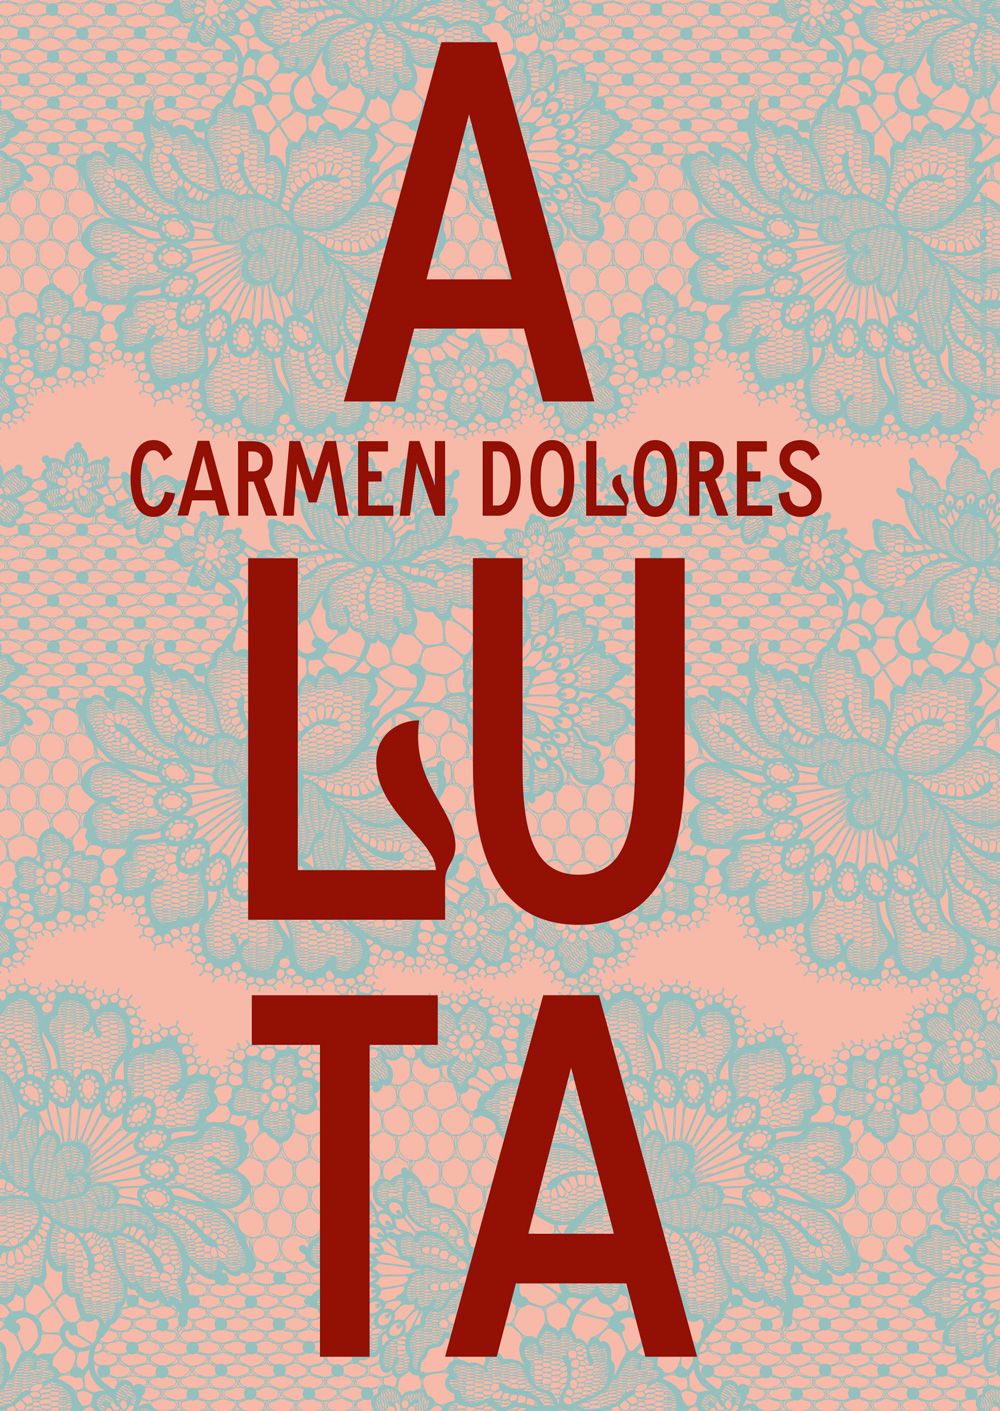
\includegraphics[width=50mm]{./imgs/luta.jpg}
\end{center}

\hspace*{-7cm}\hrulefill\hspace*{-7cm}

\medskip

\noindent{}{\slsc{A luta}} é um retrato desabusado do que era ser mulher em uma sociedade (ainda mais) dominada pelos homens, escrito por uma das mais corajosas e influentes jornalistas do começo do século 20, Carmen Dolores, pseudônimo de Emília Moncorvo Bandeira de Melo. Conta de Cecília, que se rebela contra sua vida e tenta livrar"-se das amarras patriarcais de um casamento insosso e do duplo jugo da mãe ambiciosa e da sogra conservadora.

%\hspace{.5cm}
\vfill

\hspace*{-.4cm}\begin{minipage}[c]{1\linewidth}
\small{
{\Formular{\textbf{
\hspace*{-.1cm}Título: A luta\\
Autor: Carmen Dolores\\ 
Páginas: 180\\
Formato: 14x21cm\\
Preço: R\$ 42,90\\
ISBN: 978-85-5494-620-3\\
Disponibilidade: Em breve
}}}}
\end{minipage}

\pagebreak


%\hspace{.5cm}
%
%\begin{center}
%\hspace*{-.5cm}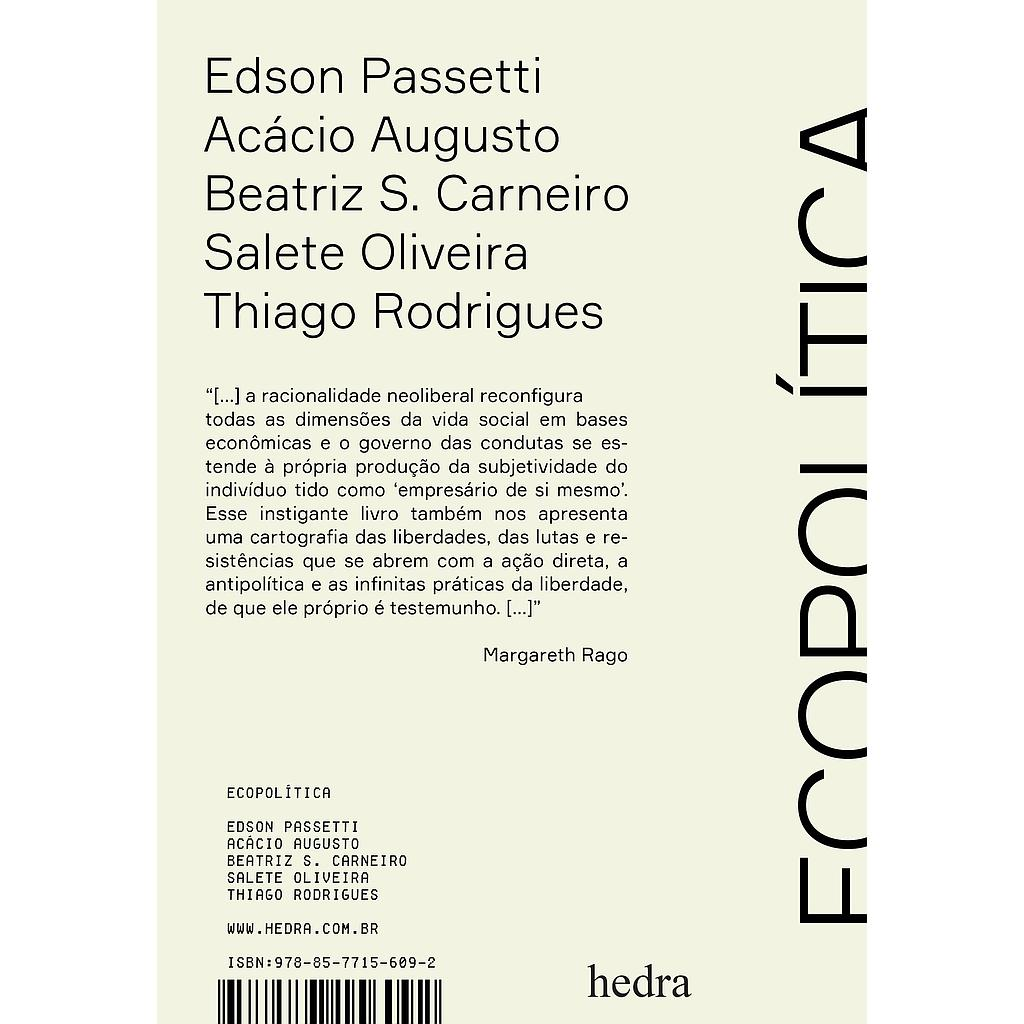
\includegraphics[width=70mm]{eco.jpeg}
%%\hspace*{6cm}\raisebox{2cm}{\rotatebox[origin=t]{90}{\Formular{\textbf{Lançamento}}}}
%\end{center}
%
%\hspace*{-2cm}\_\_\_\_\_\_\_\_\_\_\_\_\_\_\_\_\_\_\_\_\_\_\_\_\_\_\_\_\_\_\_\_\_\_\_\_\_\_\%_\_\_\_\_\_\_\_\_\_\_\_\_\_\_\_\_\_\_\_\_\_\_\_\_\_\_\_\_\_\_\_\_\_\_\_
%
%\medskip
%
%\noindent{}Lorem ipsum dolor sit amet, consectetur adipiscing elit.
%Donec sodales tortor a purus accumsan, ut ultricies purus
%maximus. Aliquam bibendum consequat mi, sed commo-
%do velit pellentesque id. Vivamus ultricies ligula in semper
%sagittis. Donec mollis odio in lectus tristique, sed convallis
%est interdum. Cras eget sem condimentum, pretium purus
%eu, auctor.
%
%\hspace{.5cm}
%
%\hspace*{-.4cm}\begin{minipage}[c]{0.45\linewidth}
%\small{
%{\Formular{\textbf{
%\hspace*{-.1cm}Título: Ecopolítica\\
%Autor: Edson Passetti\\ 
%Editora: Hedra\\
%Páginas: 476\\
%Formato: 23x16cm\\
%Preço: R\$ 79,90\\
%}}}}
%\end{minipage}
%\begin{minipage}[c]{0.50\linewidth}
%\small{Lorem ipsum dolor sit amet, consectetur adipiscing elit. onec sodales tortor a purus accumsan, ut ultricies. Lorem ipsum dolor sit amet, %consectetur adipiscing elit. Lorem ipsum dolor sit amet. Lorem ipsum dolor sit amet.} 
%\end{minipage}